\chapter{Methods}

\section{Datasets}
In this section, we introduce some important datasets used in this thesis for model training and performance evaluation. The most interesting dataset in the context of the research of this project is the 3D+t dataset of zebrafish embryo provided by the biologists at @todo.
There are multiple challenges when working with these datasets. The most important challenge is the lack of annotated data. Even for fully annotated datasets, inter-annotator agreement is often an upper boundary for evaluation, as even for the specialist a clear annotation is sometimes not obvious. This can be due to a certain level of noise in the images or boundaries that are just inherently hard to define due to the cell type or imaging modality. This is especially the case for the non-synthetic data, provided by the Celltracking Challenge (CTC) \cite{ctc}. Next to limited annotations, 3D data can quickly blow up computational resources due to their large size. For this matter, some shifted window approach has to be considered, if the image size exceeds computational limits. Anisotropy can also can also lead to distortions in feature aquisition and performance impairments at inference, if not taken care of in each processing step. 
\section{Mediar3D}

In this section, we introduce a way of extending Mediar to 3D. First, we present a way of using predictions along different image reslices, to compute a 3D flow field, which can be post processed into 3D predictions. We will briefly introduce challenges that go along with this method and discuss the feasibility of extending Mediar to true 3D. This would correspond to an architecture that learns actual 3D features during training.

\subsection{3D Flowfield Prediction}

For the extention to 3D flow predictions, we adapt the flow accumulation of Cellpose. 

\begin{figure}[!ht]
    \centering
    \makebox[\textwidth]{%
    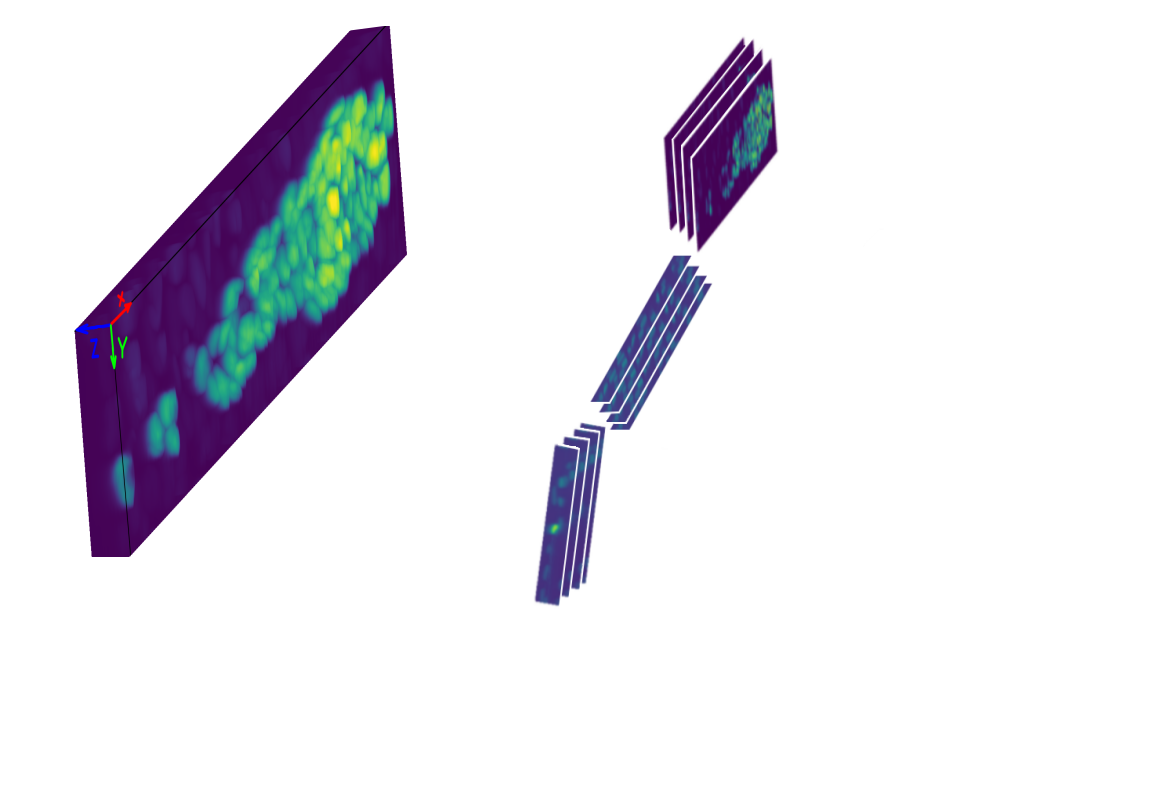
\includegraphics[width=1.0\textwidth]{Images/Methods/slicing_zebra.png}%
    }
    \caption{Encoder embeddings of the train set clustered with k-mean and intuition of amlplified sampling \cite{LeCun.1989}.}
    \label{fig:slicing}
\end{figure}

\section{Hiera3D}


\section{Training Challenges and Solutions}


\section{3D Feature Network}




